\documentclass[twosided,a4,10pt]{article}
\usepackage[utf8]{inputenc}
\usepackage{amsmath}
\usepackage{amsfonts}
\usepackage{amssymb}
\usepackage{textcomp}
\usepackage{german}
\usepackage{graphicx}
\usepackage[usenames,dvipsnames]{xcolor}
\usepackage{pifont}
\usepackage{nicefrac}
\usepackage{sectsty}

% ------
% Fonts and typesetting settings
\usepackage[sc]{mathpazo}
\usepackage[T1]{fontenc}
\linespread{1.1} % Palatino needs more space between lines
\usepackage{microtype}
\subsectionfont{\fontsize{10}{15}\selectfont}

% ------
% Page layout
\usepackage[hmarginratio=1:1,top=32mm,columnsep=20pt]{geometry}
\usepackage[font=it]{caption}
\usepackage{paralist}
\usepackage{multicol}

%------
%caption hack
\usepackage{caption}

\DeclareCaptionType{faltung}[][List of equations]
\captionsetup[faltung]{labelformat=empty}

% ------
% Abstract
\usepackage{abstract}
	\renewcommand{\abstractnamefont}{\normalfont\bfseries}
	\renewcommand{\abstracttextfont}{\normalfont\small\itshape}


% ------
% Titling (section/subsection)
\usepackage{titlesec}
%\renewcommand\thesection{\Roman{section}}
\titleformat{\section}[block]{\large\scshape\centering}{\thesection.}{1em}{}

% ------
% Clickable URLs (optional)
\usepackage{hyperref}

% ------
% Header/footer
\usepackage{fancyhdr}
	\pagestyle{fancy}
%	\fancyhead{}
%	\fancyfoot[C]{WIS WS 2017/18 $\cdot$
%          Software Engineering $\cdot$ Prof. Dr. Dünnweber}
	\fancyhead[C]{OTH Regensburg $\cdot$ Fakultät IM}
%	\fancyfoot[RO,LE]{\thepage}
	\fancyfoot[L]{WIS $\cdot$ WS 2017/18}
	\fancyfoot[R]{Prof. Dr. Dünnweber}
	\fancyfoot[C]{\thepage}


% ------
% Maketitle metadata
\title{\vspace{-5mm}%
	\fontsize{20pt}{10pt}\selectfont
	\textbf{Inhaltsbasierte Musikempfehlung mit Convolutional Neuronalen Netzwerken}
	}	
\vspace{-5mm}\date{}
\author{
	\large
       \begin{minipage}[t]{0.5\linewidth}
         \begin{center}
           	\textsc{Weidhas Philipp}\\[2mm]
                 \normalsize	Matr.nr: 123456\\
                 \normalsize
                 \href{mailto:philipp.weidhas@st.oth-regensburg.de}
                 {philipp.weidhas@st.oth-regensburg.de}      
         \end{center}
       \end{minipage}        
       \begin{minipage}[t]{0.5\linewidth}
         \begin{center}
           	\textsc{Wildgruber Markus}\\[2mm]
                 \normalsize	Matr.nr: 123456\\
                 \normalsize
                 \href{mailto:markus.wildgruber@stud.oth-regensburg.de}
                 {markus.wildgruber@stud.oth-regensburg.de}      
         \end{center}
       \end{minipage}
     }




%%%%%%%%%%%%%%%%%%%%%%%%
\begin{document}

\maketitle
\thispagestyle{fancy}

	

\begin{multicols}{2}

\begin{abstract}
\noindent Hier kommt die Zusammenfassung...
\end{abstract}


\section{Einleitung}

\section{Bestehende Ansätze zur Problemlösung}
Zur Lösung des in der Einleitung erläuterten Problems, gibt es bereits mehrere erprobte und in verschiedenster Weise angewandte Problemlösungsansätze. Diese Ansätze werden in diesem Kapitel nun eingehend erläutert. Im genauen werden aktuell 3 verschiedene Verfahren angewandt, diese sind ein inhaltsbezogener Ansatz, ein Kontextbasierenender Ansatz und ein Hybrides Verfahren das beide Verfahren in sich vereint.
\subsection{Inhaltsbasierter Filter}
TODO: Inhaltsbasierend, Inhaltsbezogen ist meiner Meinung nach der Falsche ausdruck dafür! :TODO
Als erstes wird nun ein genauerer Blick auf den inhaltsbezogenen Ansatz geworfen. Mittels diesem Verfahrens werden Nutze Musikstücke aufgrund aus Lieder gewonnener Informationen vorgeschlagen. Dies bedeutet im Detail dass aus den Musikstücken mittels verschiedenster Metriken die Audio Signale eines Liedes analysiert werden um Erkenntnisse über die Stimmung eines Liedes, die Frequenz oder Rythmus zu erhalten. Auf Grund dieser Informationen können Stücke dem Konsumenten vorgeschlagen werden die einen gleichen oder sehr ähnlichen Inhalt bieten.
\subsection{Kontextbasierter Filter}
Das zweite Verfahren welches nun eingehender betrachtet wird, ist ein kontextbasiertes Verfahren. Im diesen Verfahren wird der Ansatz verfolgt das Lieder einem Nutzer auf Grundlage von Nutzungsverhalten anderer Anwender der gleichen Plattform vorgeschlagen werden. In der Praktischen Umsetzung bedeutet dies, hört ein Anwender ein bestimmtes Musikstück wird im vom System, Lieder vorgeschlagen welche Nutzer in Zeitraum davor nach diesem diesem Stück hörten. Dieses Verfahren geht davon aus das durch die Verbindung der Lieder durch vorhergehende Aufrufe eine gute Aussage darüber getroffen werden kann wie gut diese Stücke zusammen passen. Werden Lieder häufig Nacheinander gehört, wird diese Verbindung höher bewertet und die Empfehlung häufiger ausgesprochen. Auch wird das Verhalten und der Musikgeschmack des Kunden selbst analysiert um so über Ähnlichkeiten der Kundenpräferenzen mit derer anderer, diesen wiederum bessere Empfehlungen aussprechen zu können. So werden Lieder einem Musikstil zugeordnet und so zielgerichtet dem Nutzer nahegelegt.
\subsection{Hybrider Ansatz}

\section{Convolutional Neuronale Netzwerke}
Nachdem Alex Krizhevsky mit seinem Team den ImageNet ILSVRc-2012 Kontest mit Hilfe eines tiefen Neuronalen Netzwerks (DNN) gewann. Wurden DNNs auch in anderen Bereichen neben der Bildklassifizierung \cite{alex}  in Gesichtserkennung \cite{ding}, Spracherkennung \cite{graves} und der Inhaltsbasierten Musikempfehlung \cite{oord} mehr genutzt und erforscht.\newline
Um diese unterschiedliche Funktionalität zu lernen, werden DNN mit drei verschiedenen Arten trainiert. Dem überwachten Lernen (supervised learning) bei dem das DNN eine Eingabe erhält, dessen Ausgabe bekannt ist. Durch das Vergleichen der Netzwerkausgabe mit der Erwarteten, kann das DNN dementsprechend konfiguriert werden. Beim Unüberwachten Lernen (unsupervised learning) erhält das DNN verschiedene Eingaben und soll selbständig zusammenhänge zwischen diesen erkennen. Beim bestärkten Lernen (reinforcement learning) befindet sich das DNN in einer ihm unbekannter Umgebung, die es zu erforschen gilt. Gewünschtes Verhalten wird belohnt, wodurch es lernt die richtigen Entscheidungen zu treffen \cite{wang2}.\newline 
Vorallem in den letzen Jahren hat sich das Convolutional Neuronales Netzwerk (CNN) als das erfolgsversprechendste DNN erwiesen.\newline 
Im folgenden Absatz wird eine Übersicht über den Aufbau, das Training und die Besonderheiten eines CNNs dargelegt. Anschließend werden verschiedene Ansätze der Inhaltbasierten Musikempfehlung miteinander verglichen.

\subsection{Aufbau eines Convolutional Neuronalen Netzes}
Im Unterschied zu reglären DNN verwedet das CNN Neuronen, die drei Dimensionale angeordnete sind. Durch diese Anordnung ist es möglich größere Inputdaten in der selben Geschwindigkeit zu verarbeiten wie zuvor \cite{karpathy}. Um eine CNN Architektur zu erstellen werden drei Haupttypen von Schichten verwendet: Faltungs- (convolutional layer), Vereinigungs- (pooling layer) und einer vollständig verbundenen Schicht (fully-connected layer).

\subsubsection*{Faltungsschicht}
Jede Faltungsschicht besteht aus einem oder mehreren lernfähigen Filtern. Jeder dieser Filter ist räumlich kleiner (Höhe und Breite) aber erstreck sich über die selbe Tiefe der Eingangsmatrix. Durch die Iteration über jeden Punkt in der Eingabematrix erstellt die Faltungsschicht eine zweidimensionale Aktivierungskarte. Anhand dieser erkennt die Schicht dann gewünschte Merkmale wieder \cite{karpathy}.\newline
Sei die Eingabematrix I eine 7x7x3 Matrix und K ein 3x3x3 Filter. So wird in der Ausgabematrix S die Stelle (i,j) durch die Gleichung (\ref{faltung1})  berechnet. Eine genauere Herleitung der Gleichung findet der Leser u. a. bei Goodfellow \cite{goodfellow}(328f). Die Faltung wird in Abbildung \ref{img:faltung} dargestellt.
\begin{equation}\label{faltung1}
S(i,j) =(I*K)(i,j)
\end{equation}
\begin{equation}\label{faltung2}
(I*K)(i,j) =\newline\sum_{m}^{}\sum_{n}^{}I(i+m,j+n)K(m,n)
\end{equation}
Gleichung (\ref{faltung2}) zeigt eigentlich Cross-Correlation wird aber oft auch als Faltung bezeichent \cite{goodfellow}(328)\\
\\
\begin{minipage}{0.45\textwidth}
	\centering
	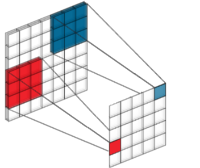
\includegraphics{img/faltung-klein.png}
	\captionof{figure}{Faltung eine 7x7x3 Matrix mit einem 3x3x3 Filter und erzeugter Aktivierungskarte \cite{knupp}}
	\label{img:faltung}
\end{minipage}

\subsubsection*{Verbindungsschicht}
Üblicherweise wird eine Verbindungsschicht zwischen zwei Faltungschichten eingefügt. Seine Funktionbesteht darin, schrittweise die Größe der Darstellung zu reduzieren, um die Anzahl der Parameter und dadurch die Berechnung des gesammt Netwerkes zu verringern \cite{karpathy}. Sie ersetzt die Ausgabe eines Netzes an einem bestimmten Punkt durch eine statistische Zusammenfassung der nahegelegenen Ausgängen. Zum Beispiel Max Pooling \cite{zhou} Übergabe der größte Zahl in einem rechteckigen Umfeld, Durchschnittsberechnung des Umfeldes oder ein gewichteter Durschnitt basierend auf die Entfernung eines zentralen Punktes \cite{goodfellow}(355).

\subsubsection*{Vollständig verbundenen Schicht}
Neuronen in einer vollständig verbundenen Schicht haben Verbindungen zu allen Knoten der vorherigen Schicht. Ihre Aktivierung wird durch eine Matrixmultipliklation und einem Bias-Offset berechnet \cite{karpathy}. Die vollständig verbundenen Schicht wird als Ausgabeschicht verwendet um aus der Eingangsmatrix einen Vektor zu erzeugen.

\subsubsection*{Training}

\subsection{Vergleich verschiedener Ansätze}

\section{Experiment}

\subsection{Aufbau}

\subsection{Ergebnis}

\section{Vergleich mit Stand der Forschung und Ausblick}

%\bibliographystyle{abbrvdin}
\bibliographystyle{unsrt}
\bibliography{lit}

\end{multicols}

\end{document}
